
\documentclass[12pt]{mitthesis}
\usepackage{titlesec}
\usepackage{geometry}
\usepackage{graphicx}
\usepackage{booktabs, chemformula}
\usepackage{titlesec, blindtext, color}
\usepackage{listings}
\usepackage{natbib}
\usepackage{float}
\usepackage{xcolor} 
\pagestyle{plain}

\begin{document}

\tableofcontents

\pagestyle{plain}

\chapter{Presentation of the research topic}

The domain of the proposed thesis is Automated Software Engineering. The thesis will develop methods for the analysis of legacy software systems, focusing on using historical information describing the evolution of the systems extracted from the versioning systems. 
The methods for analysis will integrate techniques based on computational algorithms as well as data-mining. As proof-of-concept, tool prototypes will implement the proposed methods and validate them by extensive experimentation on several cases of real-life systems.

\chapter{Software evolution and maintainability}
\section{Software evolution}
\subsection{Stages}
\label{stages}
Software has distinctive stages during its life:

\textbf{Initial development} In this stage, the first functional version of the system is developed. Also, many of the main features are developed and documented and, the architecture is defined: components that compose the system, their interactions, and properties. 

In this stage, the architecture is defined and must be made in such a manner that the software will easily support new additions. Changes made in the evolution stages must change very little the architecture defined in the initial stage \cite{model-bennett}.  The architecture must:
\begin{itemize}
\item allow unanticipated change in the software without compromising system integrity.
\item evolve in controlled ways. \cite{Bennett}
\end{itemize}

\textbf{Evolution} The evolution stage begins only after the initial stage is passed successfully. In this stage, iterative changes are made. By changes, we mean additions (new software features), modifications (changes of requirements or misunderstood requirements) or deletions. There are two main reasons for the change: the learning process of the software team and new requests from the client.

\textbf{Servicing} - Like we mentioned in the description of the initial stage, the architecture must be made in such a manner that the software may easily embrace changes. But, if not, then new changes are no longer easy to be made, are very difficult and time-consuming. At this point, the software enters the servicing stage (also called aging software, decayed software, and legacy) \cite{Software-life-cycle}, \cite{363157}.

\textbf{Phase out} - This stage is also called decline \cite{Software-life-cycle}. If in the servicing stage limited changes are implemented, in the phase-out stage the entire development is frozen. In this way the software becomes outdated. The users must make workarounds in order to cover the deficiencies of the software.

\textbf{Close down} - In this stage, the software is completely shut down, and the users redirected to a replacement system if this exists.

The stages presented above are represented in Figure \ref{fig:stagedmodel}.

\begin{figure}[H]
\centering
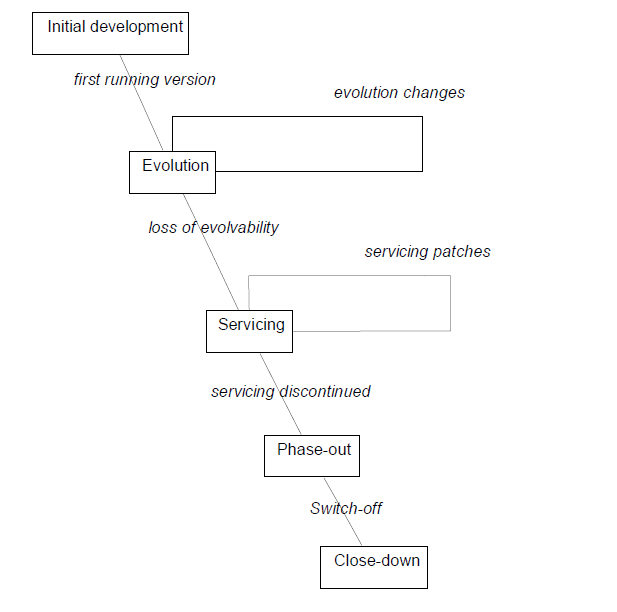
\includegraphics[width=\textwidth]{staged_model.png}
\label{fig:stagedmodel}
\caption{The versioned staged model \cite{model-bennett}}
\end{figure}

\subsection{Software change}
\label{change}
As mentioned in section \ref{stages}, software change in made in evolution and servicing stages. The difference between changes made in the evolution stage and changes made in the servicing stage is the effort of making changes. In the evolution stage, software changes are made easily and do not require much effort while in the servicing stage only a limited number of changes are made and require a lot of effort, so are really time-consuming \cite{Bennett}, \cite{Rajlich}.

The change is triggered either by new feature requests from the client or by misunderstanding the previous requirements and re-implementing them. 

The change mini-cycle consists of the following phases \cite{810308}:
\begin{itemize}
\item Phase 1: The request for change. This usually comes from the users of the software and it can also be a bug report or a request for an additional functionality. 
\item Phase 2: The planning phase, this includes program comprehension and change impact analysis. Program comprehension is a mandatory prerequisite of the change while change
impact analysis indicates how costly the change is going to be. \cite{Bohner}
\item Phase 3: The change implementation, restructuring for change and change propagation.
\item Phase 4: Verification and validation.
\item Phase 5: Re-documentation.
\end{itemize}

\section{Software maintenance}
In early days software maintenance was a small part of the software life cycle. As time was passing and more software was created, people realized that software does not die. Even if the actual development of the software may be frozen, requests regarding bug fixing and compatibility with new operating systems may appear over time. Sometimes software maintenance requires more effort than to build the system from scratch \cite{Yang:2003:SES:599790}, \cite{nsbreloaded}.

Lientz and Swanson categorized maintenance activities into four classes \cite{Lientz:1981:PAS:358790.358796}:
\begin{itemize}
\item Adaptive maintenance: changes in the software environment.
\item Perfective maintenance: new user requirements and documentation improvement.
\item Corrective maintenance: debugging and bug fixing.
\item Preventive maintenance: prevent future problems.
\end{itemize}

They also made a survey on the problems of application software maintenance in 487 organizations. The survey showed that most of the maintenance effort was on the first two types (adaptive and perfective maintenance). Many other studies suggest similar results \cite{Bennett}.
All these studies underline one thing: \textit{the incorporation of new user requirements is the main problem for software evolution and maintenance} \cite{Lientz:1981:PAS:358790.358796}, \cite{Brooks:1987:NSB:26440.26441}.

One may ask why maintenance requires so much effort? There are some main problem factors when it comes to maintenance:

\begin{itemize}
\item User knowledge: lack of user training and/or lack of understanding of the system.
\item Programmer effectiveness: lack of skills or experience for maintenance, development.
\item Product quality: quality of the original system, quality of documentation and specs.
\item Machine requirements: increasing storage or decreasing processing time requirements.
\item System reliability: data integrity, hardware, and software reliability.
\end{itemize}

%%%%%%%%%%%%%%%%%%%%%%%%%%%%%%%%%%%%%%%%%%%%%%%%%%%%%%%%%%%%%%%%%%%
\chapter{Dependencies in software systems}
A dependency is created by two elements that are in a relationship and indicates that an element of the relationship, in some manner, depends on the other element of the relationship \cite{Booch:2004:OAD:975416}, \cite{Cataldo2009SoftwareDW}.

A developer gains information about a software system by looking at it in two different ways: 
\begin{itemize}
	\item top-down: starting from the highest level of abstraction of the system and going down to the code.
	\item bottom-up: starting from the code and going up to the highest level of abstraction.
\end{itemize}

Both ways imply gradually gaining new information about the system and in both, the developer traces the dependencies and connections of the software system \cite{Wilde90understandingprogram}, \cite{341244}.

\section{Structural dependencies}
Structural dependencies can be found by analyzing the source code \cite{Sangal:2005:UDM:1094811.1094824}, \cite{CalloArias2011}. 
There are several types of relationships between these source code entities and all those create \textit{structural dependencies}:

\subsubsection{Data Item Dependencies}
Data items can be variables, records or structures. A dependency is created between two data items when the value held in the first data item is used or affects the value from the second.

\subsubsection{Data Type Dependencies}
Data items are declared to be of a specific data type. Besides the built-in data types that every programming language has, developers can also create new types that they can use. Each time the data type definition is changed it will affect all the data items that are declared to be of that type. 

\subsubsection{Subprogram Dependencies}
A subprogram is a sequence of instructions that performs a certain task. Depending on the programming language a subprogram may also be called a routine, a method, a function or a procedure. When a subprogram is changed, the developer must check the effects of that change in all the places that are calling that subprogram. Subprograms may also have dependencies with the data items that they receive as input or the data items that they are computing.



\section{Logical dependencies}
\subsection{Software evolution and version control systems}
Software evolution implies change which can be triggered either by new feature requests or bug reports \cite{articleEvolution}. As presented also in section \ref{change}, one phase of the change mini-cycle consists of change implementation and propagation (changing source code files). 
Usually, developers use version control when it comes to software development. Version control is a system that records changes to a file or set of files over time so that developers can recall specific versions of those files later \cite{svn}.
Distributed version control systems (such as Git, Mercurial, Bazaar or Darcs) allows many developers to collaboratively develop their projects \cite{7471284}.

\subsection{Definition}
\textit{Logical dependencies} (a.k.a logical coupling) can be found by software history analysis and can reveal relationships that are not always present in the source code (structural dependencies).  

Software engineering practice has shown that sometimes modules which do not present structural dependencies still appear to be related. Co-evolution represents the phenomenon when one component changes in response to a change in another component \cite{Yu:2007:UCC:1231330.1231370}, \cite{5166450}. Those changes can be found in the software history maintained by the versioning system. Gall \cite{Gall:1998:DLC:850947.853338}, \cite{Gall:2003:CRH:942803.943741} identified as logical coupling between two modules the fact that these modules  \textit{repeatedly} change together during the historical evolution of the software system \cite{6606615}.

The concepts of logical coupling and logical dependencies were first used in different analysis tasks, all related to changes: for software change impact analysis \cite{1553643}, for identifying the potential ripple effects caused by software changes during software maintenance and evolution \cite{DBLP:conf/issre/OlivaG15}, \cite{Oliva:2011:ISL:2067853.2068086}, \cite{Poshyvanyk2009}, \cite{posh2010} or for their link to deffects \cite{wiese}, \cite{Zimmermann:2004:MVH:998675.999460}.

The current trend recommends that general dependency management methods and tools should also include logical dependencies besides the structural dependencies \cite{Oliva:2011:ISL:2067853.2068086}, \cite{DBLP:journals/jss/AjienkaC17}. 



\subsection{Current status of research}

Oliva and Gerosa \cite{Oliva:2011:ISL:2067853.2068086}, \cite{DBLP:conf/issre/OlivaG15} have found first that the set of co-changed classes was much larger compared to the set of structurally coupled classes. They identified structural and logical dependencies from 150000 revisions from the Apache Software Foundation SVN repository. Also they concluded  that in at least 91\% of the cases, logical dependencies involve files that are not structurally related. This implies that not all of the change dependencies are related to structural dependencies and there could be other reasons for software artifacts to be change dependent.

Ajienka and Capiluppi also studied the interplay between logical and structural coupling of software classes. In \cite{DBLP:journals/jss/AjienkaC17} they  perform experiments on 79 open source systems: for each system, they determine the sets of structural dependencies, the set of logical dependencies and the intersections of these sets. They quantify the overlapping or intersection of these sets, coming to the conclusion that not all co-changed class pairs (classes with logical dependencies) are also linked by structural dependencies. One other interesting aspect which has not been investigated by the authors in \cite{DBLP:journals/jss/AjienkaC17}  is the total number of logical dependencies, reported to the total number of structural dependencies of a software systems. However, they provide the raw data of their measurements and we calculated the ratio between the number of logical dependencies and the number of structural dependencies for all the projects analyzed by them: the average ratio resulted 12.  This means that, using their method of detecting logical dependencies for a system, the number of logical dependencies outnumbers by one order of magnitude the number of structural dependencies. We consider that such a big number of logical dependencies needs additional filtering. 


Another kind of non-structural dependencies are the semantic or conceptual dependencies \cite{Poshyvanyk2009}, \cite{posh2010}. Semantic coupling is given by the degree to which the identifiers and comments from different classes are similar to each other. Semantic coupling could be an indicator for logical dependencies, as studied by Ajienka et al in \cite{DBLP:journals/ese/AjienkaCC18}. The experiments showed that a large number of co-evolving classes do not present semantic coupling, adding to the earlier research which showed that a large number of co-evolving classes do not present structural coupling. All these experimental findings rise the question whether it is a legitimate approach to accept all co-evolving classes as logical coupling.

Zimmermann et al \cite{Zimmermann:2004:MVH:998675.999460} introduced data mining techniques to obtain association rules from version histories.
The mined association rules  have a probabilistic interpretation based on the amount of evidence in the transactions they are derived from. This amount of evidence is determined by two measures: support and confidence.  They developed a tool to predict future or missing changes.

Different applications based on dependency analysis could be improved if, beyond structural dependencies, they also take into account the hidden non-structural dependencies. For example, works  which investigate different methods for architectural reconstruction \cite{SoraConti}, \cite{SoraSem13}, \cite{PagerankENASE},  all of them based on the information provided by structural dependencies, could enrich their dependency models by taking into account also logical dependencies. However, a thorough survey \cite{sar} shows that historical information has been rarely used in architectural reconstruction. 

Another survey \cite{Shtern:2012:CMS:2332427.2332428} mentions one possible explanation why historical information have been rarely used in architectural reconstruction: the size of the extracted information. One problem is the size of the extraction process, which has to analyze many versions from the historical evolution of the system. Another problem is the big number of pairs of classes which record co-changes and how they relate to the number of pairs of classes with structural dependencies.

The software architecture is important in order to understand and maintain a system. Often code updates are made without checking or updating the architecture. This kind of updates cause the architecture to drift from the reality of the code over time \cite{sar}.
So reconstructing the architecture and verifying if still matches the reality is important \cite{Kalliamvakou2016}. 

Surveys also show that architectural reconstruction is mainly made based on structural dependencies \cite{Shtern:2012:CMS:2332427.2332428}, \cite{sar}, the main reason why historical information is rarely used in architectural reconstruction is the size of the extracted information.

Logical dependencies should integrate harmoniously with structural dependencies in an unitary dependency model: valid logical dependencies should not be omitted from the dependency model, but structural dependencies should not be engulfed by questionable logical dependencies generated by casual co-changes.  
Thus, in order to add logical dependencies besides structural dependencies in dependency models, class co-changes must be filtered until they remain only a reduced but relevant set of valid logical dependencies. 

Currently there is no set of rules or best practices that can be applied to the extracted class co-changes and can guarantee their filtering into a set of valid logical dependencies.
This is mainly because not all the updates made in the versioning system are code related. For example a commit that has as participants a big number of files can indicate that a merge with another branch or a folder renaming has been made. In this case, a series of irrelevant co-changing pairs of entities can be introduced. So, in order to exclude this kind of situations the information extracted from the versioning system has to be filtered first and then used.

Other works have tried to filter co-changes \cite{Oliva:2011:ISL:2067853.2068086}, \cite{DBLP:journals/jss/AjienkaC17}. One of the used co-changes filter is the commit size.The commit size is the number of code files changed in that particular commit. 
Ajienka and Capiluppi established a threshold of 10 for the maximum accepted size for a commit \cite{DBLP:journals/jss/AjienkaC17}. This means that all the commits that had more than 10 code files changed where discarded from the research. But setting a harcoded threshold for the commit size is debatable because in order to say that a commit is big or small you have to look first at the size of the system and at the trends from the versioning system. Even thought the best practices encourage small and often commits, the developers culture is the one that influences the most the trending size of commits from one system.

Filtering only after commit size is not enough, this type of filtering can indeed have an impact on the total number of extracted co-changes, but will only shrink the number of co-changes extracted without actually guaranteeing that the remaining ones have more relevancy and are more logical linked.

Although, some unrelated files can be updated by human error in small commits, for example: one file was forgot to be commited in the current commit and will be commited in the next one among some unrelated files. This kind of situation can introduce a set of co-changing pairs that are definitely not logical liked. In order to avoid this kind of situation a filter for the occurrence rate of co-changing pairs must be introduced. Co-changing pairs that occur multiple times are more prone to be logically dependent than the ones that occur only once. Currently there are no concrete examples of how the threshold for this type of filter can be calculated. In order to do that, incrementing the threshold by a certain step will be the start and then studying the impact on the remaining co-changing pairs for different systems. 

Taking into account also structural dependencies from all the revisions of the system was not made in previous works, this step is important in order to filter out the old, out-of-date logical dependencies. Some logical dependencies may have been also structural in previous revisions of the system but not in the current one. If we take into consideration also structural dependencies from previous revisions then the overlapping rate between logical and structural dependencies could probably increase. Another way to investigate this problem could be to study the trend of concurrences of co-changes: if co-changes between a pair of classes used to happen more often in the remote past than in the more recent past, it may be a sign that the problem causing the logical coupling has been removed in the mean time. 



\section{Extracting logical dependencies from co-changes}

Changes made to two components in the same commit do not necessarily indicate the co-evolution of the two. These changes could be completely unrelated. The study \cite{Yu2007} acknowledges the fact that evolutionary coupling could also be determined accidentally by two components changing in the same commit (independent evolution, as it is called) and this will bring noise to the measurement of evolutionary coupling. 

In order to add logical dependencies besides structural dependencies as inputs for methods and tools for dependency management and analysis, class co-changes must be filtered until they remain only a reduced but relevant set of valid logical dependencies. 

\subsection{Filtering based on the size of commit transactions}

A big commit transaction can indicate that a merge with another branch or a folder renaming has been made.
In this case, a series of irrelevant logical dependencies can be introduced since not all the files are updated in the same time for a development reason. Different works have chosen fixed threshold values for the maximum number of files accepted in a commit. Cappiluppi and Ajienka, in their works \cite{DBLP:journals/jss/AjienkaC17}, \cite{DBLP:journals/ese/AjienkaCC18} only take into consideration commits with less then 10 source code files changed in building the logical dependencies.

The research of Beck et al \cite{Beck:2011:CMC:2025113.2025162} only takes in consideration transactions with up to 25 files. The research \cite{Oliva:2011:ISL:2067853.2068086} provided also a quantitative analysis of the number of files per revision; Based on the analysis of 40,518 revisions, the mean value obtained for the number of files in a revision is 6 files. However, standard deviation value shows that the dispersion is high. 

\subsection{Filtering based on the number of occurrences}
One occurrence of a co-change between two software entities can be a valid logical dependency, but can also be a coincidence. Taking into consideration only co-changes with multiple occurrences as valid dependencies can lead to more accurate logical dependencies and more accurate results. On the other hand, if the project studied has a relatively small amount of commits, the probability to find multiple updates of the same classes in the same time can be small, so filtering after the number of occurrences can lead to filtering all the logical dependencies extracted. Giving the fact that we will study multiple projects of different sizes and number of commits, we will analyze also the impact of this filtering on different projects.

\subsection{Overlaps between structural and logical dependencies}
Logical dependency can be also a structural dependency and vice-versa, so studying the overlapping between logical and structural dependencies while filtering is important since the intention is to introduce those logical dependencies among with structural dependencies in architectural reconstruction systems. Current studies have shown a relatively small percentage of overlapping between them with and without any kind of filtering \cite{DBLP:journals/jss/AjienkaC17}. This means that a lot of non related entities update together in the versioning system, the goal here is to establish the factors that determine such a small percentage of overlapping.

%%%%%%%%%%%%%%%%%%%%%%%%%%%%%%%%%%%%%%%%%%%%%%%%%%%%%%%%%%%%%%%%%%%%%%%%

\chapter{Applications of software dependencies}

\section{Reverse engineering}
The term reverse engineering was first defined by Chikofsky and Cross \cite{ChikofskyReverse} as the \textit{"process of analyzing a system to (i) identify the system’s components and
their inter-relationships and (ii) create representations of the system in another form or at a higher level of abstraction."} 

Reverse engineering is viewed as a two step process: information extraction and abstraction. \cite{FoSEReverseEngineering} 
The firs step, information extraction, is made by source code analysis which generates dependencies between software artifacts. So, reverse engineering uses dependencies in order to create new representations of the system or provide a higher level of abstraction \cite{struct_dep}, \cite{Gueheneuc}.

\section{Architecture reconstruction}
Currently, the software systems contain tens of thousands of lines of code and are updated multiple times a day by multiple developers.  
The software architecture is important in order to understand and maintain a system. Often code updates are made without checking or updating the architecture.
This kind of updates cause the architecture to drift from the reality of the code over time. So reconstructing the architecture and verifying if still matches the reality is important. \cite{sar},\cite{PagerankENASE}, \cite{Bass-archreconstruction} ,\cite{RecoverySartipi}, \cite{model-bennett}.

\section{Identifying clones}
Research suggests that a considerable part (around 5-10\%) of the source code of large-scale software is duplicate code (“clones”). Source code is often duplicated for a variety of reasons, programmers may simply be reusing a piece of code by copy and paste or they may be “reinventing the wheel” \cite{ClonesMayrand}, \cite{clones}.
Detection and removal of clones can decrease software maintenance costs \cite{CloneDetection}, \cite{cloneKamiya}.

\section{Code smells }
Code smells have been defined by Fowler \cite{bookFowler} and describe patterns that are generally associated with bad design and bad programming practices.
Originally, code smells are used to find the places in software may need refactoring \cite{articlesmells}. Studies have found that smells may affect comprehension and possibly increase change and fault proneness \cite{5741260}, \cite{5328703}, \cite{articlefault-proneness}.
Examples of code smells:
\begin{itemize}
	\item Large Class: one class with many fields.
	\item Feature Envy:  methods that access more methods and fields of another class than of its own class.
	\item Data Class: classes that only fields and do not contain functionality.
	\item Refused Bequest: classes that leave many of the fields and methods they inherit unused
	\item Parallel Inheritance: every time you make a subclass of one class you also have to make a subclass of the other.
	\item Shotgun Surgery: one method is changing together with other methods contained other classes.
\end{itemize}

Previous studies already explored the idea of using history information in order to detect code smells \cite{6963448}. 

\section{Comprehension}
Software comprehension is the process of gaining knowledge about a software system.
An increased knowledge of the software system help activities such as bug correction, enhancement, reuse and documentation \cite{Comprehension}, \cite{1199197}, \cite{2003:XLC:851042.857028}.
Previous studies show that the proportion of resources and time allocated to maintenance may vary from 50\% to 75\% \cite{articleLientz}.
Regarding maintenance, the greatest part of the software maintenance process is the activity of understanding the
system. 
Thanking into consideration the previous statements we can say that if we want to improve software maintenance we have to improve software comprehension \cite{article-cognitive-processes}.

\section{Fault location}
Debugging software is an expensive and mostly manual process. Of all debugging activities, fault localization, is the most expensive \cite{articleDebugging}. 

Software developers locate faults in their programs using a manual process. This process begins when the developers observe failures in the program. The developers choose a set of data to inject in the system(a set of data that most likely replicate previous failures or may generate new ones) and place breakpoints using a debugger. Then they observe the system's state until an failed state is reached, and then backtrack until the fault is found. 

As we said, this process has high costs so because of this high cost, any improvement in the process can decrease the cost of debugging.\cite{fault-localization} \cite{program-failures}


\section{Error proneness}
Various studies have analyzed the connection between software metrics and software quality. \cite{544352}
Those studies have shown that modules that are most likely to contain errors can be identified based on the software error history and metrics related to the amount of data and the structural complexity of software \cite{67595}, \cite{1702015}.
The most used metrics in error prone detection are the following:
\begin{itemize}
	\item WMC (Weighted Methods per Class): is the sum of all methods weights of a class
	\item DIT (Depth of Inheritance Tree): is the maximum inheritance path from the class to the root class.
	\item RFC (Response For a Class): is the number of methods that can be executed in response to a message received by an object of a class.
	\item LCOM (Lack of Cohesion of Methods): is the lack of cohesion of the methods of a class.
	\item NOC (Number Of Children): is the number of immediate sub-classes of a class.
	\item CBO (Coupling Between Object classes): is the number of classes to which a class is coupled \cite{295895}.
\end{itemize}

WMC, NOC and DIT metrics reflect class hierarchy, CBO and RFC metric reflect class coupling and LCOM reflects cohesion.



\section{Empirical software engineering research}
Empirical research seeks to explore, describe, predict, and explain natural or social phenomena by using evidence based on observation or experience.
It involves obtaining and interpreting evidence by experimentation, surveys or observation of documents or artifacts. \cite{inproceedingsEmpirical}


 %%%%%%%%%%%%%%%%%%%%%%%%%%%%%%%%%%%%%%%%%%%%%%%%%%%%%%%%%%%%%%%%%%%%%%%%%%%%%%%%

\chapter{Research content and stages of research}

\section{Proposed research stages}
The research will be made by following the next stages of implementation:\\

\textbf{Section 1:  Development of content and tools}

\textbf{Stage 1:} Build tool to extract structural dependencies from code and co-changes from git for a given set of projects.

\textbf{Stage 2:} Find filters for the co-changes extracted, the filters can be the ones already mentioned in previous works or new ones. Establish different thresholds for those filters.

\textbf{Stage 3:} Study the impact of those filters and the corresponding thresholds on the remaining quantity of co-changes for each system.
Study the overlapping between the remaining pairs of co-changing entities and the structural dependencies extracted. \cite{enase19}

\textbf{Stage 4:} Establish a dynamic way to determine the thresholds for filters in order to fit the best each studied system. Main focus on the threshold for number of occurrences of co-changing pairs.
Use plots or other visual instruments in order to see the highest and the lowest rates for the numbers of occurrences among co-changing pairs.
Also filter those rates into normal and abnormal ones and study what was the cause of the highest rates (code or human related).

\textbf{Stage 5:} Take into account also structural dependencies from all the revisions of the system to filter out the old, out-of-date logical dependencies. 
Study how this affects the remaining number of logical dependencies.Here an extra check is needed, it can be a case in which old structural dependencies that were also logically linked to continue to be logically linked
even after the structural dependency was removed.\\


\textbf{Section 2: Usage}

\textbf{Stage 6:} Export the remaining co-changes whom at this step we can call logical dependencies and use them among structural dependencies in tools for architectural reconstruction to evaluate the improvement.

\textbf{Stage 7:} Compare the number of logical dependencies with metrics like Fan Out, Fan In, Efferent Coupling (Ce), Afferent Coupling (Ca) and study their connections.

\textbf{Stage 8:} Identify other tools that use historical information and evaluate the impact of co-changes filtering into logical dependencies for them. 

\section{Gantt chart}

\begin{figure}[H]
\centering
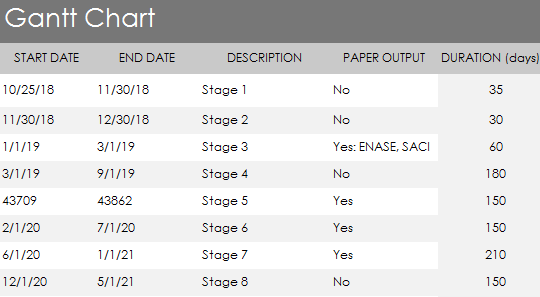
\includegraphics[width=\textwidth]{gantt_chart.PNG}
\label{fig:gantt1}
\end{figure}

\begin{figure}[H]
\centering
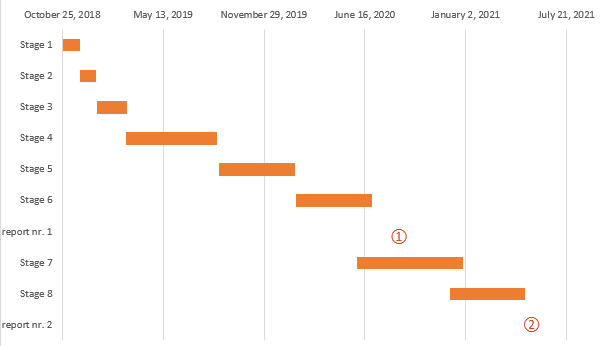
\includegraphics[width=\textwidth]{gantt_plot.PNG}
\label{fig:gantt2}
\end{figure}

\section{Proposed contents of the thesis}

 	\textbf{Chapter 1.} Introduction - This chapter will contain the motivation of the research topic and the motivation for choosing it.

\textbf{Chapter 2.} Software evolution and maintainability - This chapter will present the notions of software evolution and maintainability and the processes that those imply.

\textbf{Chapter 3.} Dependencies in software systems - This chapter will present existing types of dependencies in software systems and their nature.

\textbf{Chapter 4.} Filtering co-changes into logical dependencies - This chapter will present methods and experiments in filtering co-changes in order to obtain logical dependencies.

\textbf{Chapter 5.} Logical dependencies in practice - This chapter will present a series of applications of logical dependencies extracted from software systems.

\textbf{Chapter 6.} Conclusions - This chapter will provide the final conclusions and will summarize the contributions realized through this paper.

\bibliographystyle{plain}
\bibliography{logicaldepd}
\end{document}

